\documentclass[a4paper,12pt]{report}

\usepackage[latin1]{inputenc}
\usepackage[T1]{fontenc}
\usepackage[english,frenchb]{babel}
\usepackage[top=4cm, bottom=2cm, left=3cm, right=3cm]{geometry}
\usepackage{url}
\usepackage{graphicx}
\usepackage{float}
\usepackage{hyperref}
\usepackage{indentfirst}
\usepackage{eurosym}
\usepackage{gensymb}
\usepackage{multicol}
\usepackage{lscape}
\usepackage{amsmath}
\usepackage{array}
\usepackage{caption} % allow new line inside caption
\usepackage{subcaption}
\usepackage[toc,page]{appendix} 
\usepackage{tikz}
\usetikzlibrary{trees}
\tikzstyle{every node}=[draw=black,thick,anchor=west]
\tikzstyle{folder}=[dashed,thick]
\tikzstyle{package}=[draw=black,fill=gray!50]

% Sam's template
\usepackage{palatino}
\usepackage{phdthesis}

\hypersetup{
  backref=true,    %permet d'ajouter des liens dans...
  pagebackref=true,%...les bibliographies
  hyperindex=true, %ajoute des liens dans les index.
  colorlinks=true, %colorise les liens
  breaklinks=true, %permet le retour à la ligne dans les liens trop longs
  urlcolor= blue,  %couleur des hyperliens
  linkcolor= black, %couleur des liens internes
  bookmarks=true,  %créé des signets pour Acrobat
  bookmarksopen=true,            %si les signets Acrobat sont créés,
  %les afficher complètement.
  pdftitle={Rapport de Projet IA54}, %informations apparaissant dans
  pdfauthor={Lucie BOUTOU & Théophile Madet},     %dans les informations du document
  pdfsubject={Simulateur de traffic}          %sous Acrobat.
  }

\title{Rapport de Projet IA54 \\ Simulateur de traffic}
\author{Lucie BOUTOU \\ Théophile MADET}
\date{\today}

% un boite pour l ’auteur de la citation
\newsavebox{\auteurcitation}
\newsavebox{\boitecitation}
\newenvironment{unecitation}[1]{% clause begin
  % on sauve l ’argument 1 pour l ’auteur
  \savebox{\auteurcitation}{#1}%
\begin{lrbox}{\boitecitation}
\begin{minipage}{0.8\linewidth}%
\setlength{\parindent}{10pt}%
\large\slshape`` \ignorespaces}% on passe en petit et penché
{ ''
  \par\mbox{}\hfill\usebox{\auteurcitation}
\end{minipage}
\end{lrbox}
\begin{center}
\usebox{\boitecitation}
\end{center}}



\begin{document}
\setcounter{page}{2}
\tableofcontents

\newpage

\chapter{Introduction}

Dans le cadre de l'UV IA54 (Systèmes multi agents et résolution distribuée de problèmes), nous avons dû réaliser un simulateur de traffic, à l'aide des bibliothèques Janus et Jaak. Différents objectifs étaient proposés au cours de la réalisation de ce projet :\\
\begin{itemize}
 \item[-] réaliser le simulateur de traffic en langage Java,
 \item[-] étendre la bibliothèque Jaak afin de lui permettre d'être utilisée avec certains langages de scripts,
 \item[-] implanter dans le simulateur des agents développés dans un langage de script choisi.\\
\end{itemize}

Ce rapport présente dans une première partie les outils utilisés au cours du développement de ce projet. Dans une seconde partie, nous expliquons la manière dont nous avons réalisé le simulateur de traffic. Nous proposons dans une troisième partie une extension de la bibliothèque Jaak afin d'y intégrer les langages de script. Enfin nous concluons sur les résultats obtenus ainsi que les améliorations possibles à apporter au projet.

\chapter{Outils utilisés}

Notre simulateur de traffic doit être implémenté à l'aide de deux bibliothèques : Janus et Jaak.\\

Janus est une plateforme multi-agent open source implémentée en langage Java (version 1.6). Elle fournie des fonctionnalités permettant de développer, lancer, afficher et suivre des applications basées multi-agent. Janus peut être utilisée comme plateforme agent-orientée, plateforme organisationnelle, ou plateforme holonique. Elle est construite selon les normes du modèle organisationnel CRIO. Enfin Janus est libre pour une utilisation non commerciale et distribuée sous les termes de la licence GPLv3.\\

Jaak est un outil qui complète la bibliothèque Janus. Il fournit un environnement 2D discret ainsi que des interactions simplifiées basées sur les primitives du langages Logo. Dans Jaak, un agent est appelé tortue, comme référence à la tortue du langage Logo. Cet outil est particulièrement adapté à la modélisation de systèmes complexes se développant au cours du temps. \\

\chapter{Simulateur de traffic}

\section{Architeture générale}

L'architecture de notre application de simulation de traffic est divisée en 5 packages : \\

\begin{tikzpicture}[%
  grow via three points={one child at (0.5,-0.7) and
  two children at (0.5,-0.7) and (0.5,-1.4)},
  edge from parent path={(\tikzparentnode.south) |- (\tikzchildnode.west)}]
  \node[folder] {root}
    child {node [folder] {src}
      child { node [package] {main}
	child { node {MainProgram.java}}
      }
      child [missing] {}
      child { node [package]{environment}
	child { node {TrafficLight.java}}
	child { node {Wall.java}}
	child { node {TrafficSimulatorWorldSpawner.java}}
      }
      child [missing] {}
      child [missing] {}
      child [missing] {}
      child { node [package]{agents}
	child { node {Car.java}}
	child { node {JythonCar.java}}
      }
      child [missing] {}
      child [missing] {}
      child { node [package] {ui}
	child { node {TrafficSimulatorFrame.java}}
	child { node {TrafficSimulatorPanel.java}}
      }
      child [missing] {}
      child [missing] {}
      child { node [package] {script}
	child { node {ScriptedTurtle.java}}
	child { node {JythonTurtle.java}}
      }
    }
  child [missing] {}
  child [missing] {}
  child [missing] {}
  child [missing] {}
  child [missing] {}
  child [missing] {}
  child [missing] {}
  child [missing] {}
  child [missing] {}
  child [missing] {}
  child [missing] {}
  child [missing] {}
  child [missing] {}
  child [missing] {}
  child [missing] {}
  child {node [folder] {res}
    child {node {PythonCar.py}}
  };
\end{tikzpicture}

Le lanceur \emph{MainProgram.java} est à l'origine de la création de l'interface ainsi que de l'environnement. \\

L'environnement est composé de différents objets tels que les murs et les feux tricolores. Il contient aussi le spawner qui sera responsable de la création des tortues dans l'application.\\

Dans notre application, les tortues sont des voitures. Il existe une version de la voiture écrite en Java (à des fins de test de l'application), ainsi qu'une version écrite dans le langage de script de notre choix sur laquelle nous reviendrons dans la suite de ce rapport. \\

L'interface est uniquement composée d'une fenêtre ainsi que d'un panel, basés sur la bibliothèque Swing. \\

Un dernier package, \emph{script}, contient les classes ayant permis d'étendre Jaak à l'utilisation de langages de scripts. \\

Enfin les scripts sont stockés dans un dossier de ressources.

\section{Environnement}

Notre environnement est un espace discret 2D représenté par une grille qui dans chaque casela composant, peut contenir différentes objets et/ou tortues. \\

\begin{figure}[H]
   \centering
   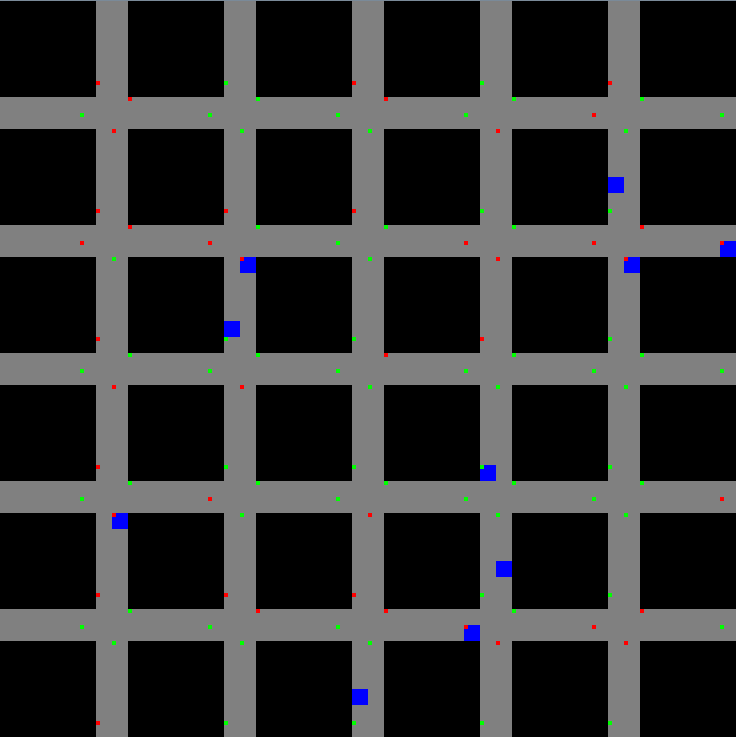
\includegraphics[scale=0.35]{environnement.png}
\end{figure}

Parmi ces objets, notre environnement possède des murs, qui sont des obstacles : cela signifie qu'aucun autre élément ne peut se trouver dans une case où se trouve déjà un mur. Les routes apparaissent donc aux endroits où il n'y a pas de murs de placés. \\

Un second objet compose notre environnement : il s'agit des feux de circulation. Cette catégorie d'objet ne correspond pas un obstacle. Il permet donc aux voitures de se déplacer sur une case comportant un feu de circulation. Néanmoins ces feux agissent sur le dépacement des voitures : lorsque le feu est rouge, les voitures ne peuvent pas progresser au delà de celui-ci. Lorsque le feu est vert, elles le peuvent. \\

La création de l'environnement se déroule dans la fonction \emph{createEnvironment} de la classe \emph{MainProgram}. Pour chaque case de la grille on lui applique le ou les objets que l'on souhaite aux coordonnées correspondantes. \\

La création des voitures est géré au sein de la classe \emph{TrafficSimulatorWorldSpawner}. Cette classe possède deux arguments importants : 
\begin{itemize}
\item[-] le nombre de voitures dont la simulation disposera,
\item[-] l'environnement créé précedemment.
\end{itemize}

Ainsi tant que le nombre de voitures dans la simulation n'est pas atteint, le spawner créé une nouvelle voiture qu'il positionne sur une case de la grille ne contenant pas de murs.

\section{Tortue}

Comme dit dans la section précédente, dans notre simulateur de traffic, les tortues proposées dans la bibliothèques Jaak sont des voitures. \\

Ces voitures peuvent se déplacer sur les routes. Pour chaque route deux voies sont disponibles pour chaque sens de circulation. Les voitures doivent se déplacer sur la voie de droite. Elles doivent également respecter les feux de circulation situés au niveau des croisements. \\

A leur création, les voitures se voient attribuer une destination aléatoirement. Leur objectif est d'atteindre cette destination, pour ensuite s'en voir attribuer une nouvelle. \\

Le déplacement des voitures est géré au sein de la fonction \emph{turtleBehaviour} qui est appelé à chaque pas de simulation. La voiture ne peut effectuer qu'un unique déplacement par pas de simulation : dès qu'un appel à la fonction \emph{move(x,y)} est réalisé au sein de la fonction \emph{turtleBehaviour}, on ne poursuit pas le déroulement de la fonction. \\

Deux cas sont considérés lors du déplacement de la voiture :
\begin{itemize}
\item[-] le parcours d'une route,
\item[-] l'intersection. \\
\end{itemize}

La voiture détecte qu'elle se trouve le long d'une route si celle ci trouve dans une de ses cases adjacentes un mur. Dans ce cas elle cherche dans quelle case se trouve le mur afin de déterminer dans quelle direction elle doit avancer. Tant que la voiture ne se trouve pas sur une intersection celle ci continue d'avancer dans la direction définie. \\

C'est uniquement lorsque la voiture se trouve sur une intersection que celle-ci va prendre une décision sur la direction qui lui parait la meilleure pour atteindre sa destination. Elle peut :
\begin{itemize}
\item[-] traverser l'intersection sans changer de direction,
\item[-] tourner sur sa droite,
\item[-] faire un demi-tour (pas en diagonale) afin de faire face à cette intersection dans le sens inverse.\\
\end{itemize}

Afin de prendre sa décision, la voiture a accès à sa position absolue (coordonnées x et y), la position de sa destination (coordonnées x et y), et sa position dans le croisement. Cette dernière information permet, une fois la direction choisie, de s'engager dans la bonne voie et éviter de rouler à contre sens.

\section{Interface}

L'interface proposée pour visualiser la simulation est bassée sur les classes \emph{JFrame} et \emph{JPanel} de la bibliothèqe Swing. \\

La fenêtre est basique, elle possède un listener pour réagir à la fermeture de celle-ci et ainsi tuer les kernels au moment de la fermeture.\\

Un panel compose cette fenêtre, c'est sur celui ci que ce sera dessiner la simulation. A chaque appel à la fonction de dessin du panel, un parcours de la grille de l'environnement est effectué, et selon l'objet ou la tortue trouvée on dessine un symbole correspondant à la bonne position :
\begin{itemize}
\item[-]un carré noir représente un mur,
\item[-]un carré rouge ou vert représente un feu de circulation,
\item[-]un carré bleu représente une voiture,
\item[-]un carré gris représente une case vide (dessiné en gris afin de le différencier de la couleur de fond du panel).
\end{itemize}


\chapter{Extension aux langages de scripts}

\section{Extension de Jaak}

Le second objectif du projet, après avoir développer le simulateur de traffic sous Java, a été d'étendre la bibliothèque Jaak afin de permettre de développer des tortues dans un certain langage de script qui pourraient ensuite être implanter dans le simulateur développé en Java. \\

Pour cela nous avons pu nous inspiré de la classe \emph{ScriptedAgent} disponible dans la bibliothèque Janus qui réalise déjà cette tâche pour implanter des agents écrits dans un certain lanage de script. \\

Sur cet exemple nous avons écrit la classe \emph{ScriptedTurtle}. Cette classe définit les noms de fonctions qui pourront être définies au sein du script correspondant à une tortue :
\begin{itemize}
 \item[-]activateTurtle,
 \item[-]behaviourTurtle,
 \item[-]endTurtle.\\
\end{itemize}

Afin de coder une tortue en langage de script, un script devra contenir au minimum la définition de la fonction behaviourTurtle.

Cette classe est la classe mère qui permet d'écrire des tortues dans un langage de script. Un template est utilisé pour définir l'interpréteur et le loader de script. \\

Il faut ensuite créé une classe personnalisée selon le langage de script choisi. Dans notre cas nous avons choisi le langage de script Python. Nous avons donc créé une classe \emph{JythonTurtle}. C'est dans celle-ci que sera spécifiée l'interpréteur et le script loader à utiliser.

\section{Voiture Python}

Après avoir obtenu la possibbilité de créer des tortues à partir du langage de script Python, il était nécessaire de créer une classe s'adaptant à notre voiture : la classe \emph{JythonCar}.\\

Cette classe ajoute à la classe \emph{JythonTurtle} des attributs et fonctions spécifiques à notre voiture, qui seront ainsi accessible au sein du script \emph{PythonCar}. C'est au sein du constructeur de la classe \emph{JythonCar} que le script est atttribué à la tortue.

Le script Python constitue principalement une traduction de la fonction turtleBehaviour que l'on trouve dans la classe \emph{Car} de la version Java de notre voiture. \\

Deux fonctions ont été ajoutées à la classe \emph{JythonCar} afin de rendre leur appel accesible au sein du script. Ces fonctions permettent de faire une traduction entre certains objets de types primitifs (int, float) compatibles entre Python et Java, vers des types complexes (Vector2f(x,y),Point2i) qui ne peuvent être créé simplement au sein d'un script Python :

\begin{verbatim}
public void setDestination(int x, int y) {
    this.destination.setX(x);
    this.destination.setY(y);
}
\end{verbatim}

\chapter{Conclusion}

Nous avons réalisé au sein de ce projet un simulateur de traffic basique, auquel pourrait être ajouté de nombreuses et variées options afin de rendre celui ci le plus réaliste possible. \\

Nous ne nous sommes pas attardés sur ce côté du projet car nous voulions nous assurer de faire fonctionner l'implantation de tortues écrites dans un langage de programmation au sein de notre simulateur. \\

Nous avons mis en place l'implantation de tortues écrites dans le langage de script Python. Il serait maintenant rapide de mettre en place la gestion d'autres langages de scripts.\\

\end{document}
